\documentclass{article}

\usepackage{rtex}
\usepackage{tikz}
\usepackage{circuitikz}
\usepackage{enumitem}
\usepackage{minted}
\usepackage{fontspec}
\usepackage[letterpaper, portrait, margin=1in]{geometry}
\setmonofont{Jetbrains Mono}

\begin{document}

\rtitle{MECH 466 Summary}{Reese Critchlow}

\header{Second-Order Systems}

For a system for which the transfer function takes on the form:
\begin{align*}
  G(s) = \frac{X(s)}{F(s)} = \frac{1}{ms^2 + Ds + k},
\end{align*}
or in the time domain:
\begin{align*}
  m\ddot{x} + D\dot{x} + kx = f(t)
\end{align*}
we can extract key parameters.
\gap
\mheader{Solving Second Order ODEs}
In the time domain, we can we can decompose the problem into a homogenous and a particular solution:
\begin{align*}
  x(t) = x_p(t) + x_c(t)
\end{align*}
and then just solve accordingly. However, in most cases, we will be analyzing the step
response of systems. Generally, this comes in the following form:
\begin{align*}
  \ddot{x} + 2\zeta \omega_n \dot{x} + \omega_n^2 = \frac{k}{m}u(t).
\end{align*}
Or, in the frequency domain:
\begin{align*}
  X(s) = \frac{\omega_n^2}{s(s^2 + 2\zeta \omega_n s + \omega_n^2)},
\end{align*}
given that $\ds \omega_n = \sqrt{\frac{k}{m}}$. All of these systems have (rougly) the following form of solution in the time domain:
\begin{align*}
  x(t) = Ae^{s_1t} + Be^{s_2t}
\end{align*}

Hence, from this, we get four following
response types:
\begin{enumerate}
\item \underline{Undamped:} $\zeta = 0$
  \gap
  $\ds s^2 + w_n^2 = 0 \implies s_{1, 2} = \pm j \omega_n$
  \gap
  $\implies x(t) = 1 - \cos(\omega_n t)$.
\item \underline{Overdamped:} $\zeta > 1$
  \gap
  $\ds s_{1, 2} = -\zeta \omega_n  \pm \omega_n \sqrt{\zeta^2 -1}$
  \gap
  $\ds \implies x(t) = 1 + Ae^{s_1t} + Be^{s_2t}$
\item \underline{Critical Damping:} $\zeta = 1$
  \gap
  $\ds s_{1, 2} = -\zeta \omega_n$
  \gap
  $\ds \implies x(t) = 1 + (A + Bt)e^{-\zeta \omega_n t}$
\item \underline{Underdamped:} $\zeta < 1$
  \gap
  $\ds s_{1, 2} = -\zeta \omega_n \pm j \omega_n \sqrt{1 - \zeta^2}$
  \gap
  $\ds \implies x(t) = 1 - \frac{e^{-\zeta \omega_n t}}{\sqrt{1- \zeta^2}}\cos \left(\omega_d t - \phi\right) $\gap
  where: $\ds \phi = \arctan \left(\frac{\zeta}{\sqrt{1-\zeta^2}}\right)$ and $\omega_d = \omega_n \sqrt{1-\zeta^2}$.
\end{enumerate}

From all of these parameters, we can extract the following metrics:
\begin{itemize}
\item \sheader{Peak Time} $\ds \tau_p = \frac{\pi}{\omega_d}$
\item \sheader{Settling Time} $\ds \tau_p = \frac{4}{\zeta \omega_n}$
\item \sheader{Percentage Overshoot} $\ds \%\text{OS} = 100e^{-\frac{\pi \zeta}{\sqrt{1-\zeta^2}}}$
\end{itemize}
From this, we can extract the following information about our system on pole graphs:
\begin{center}
  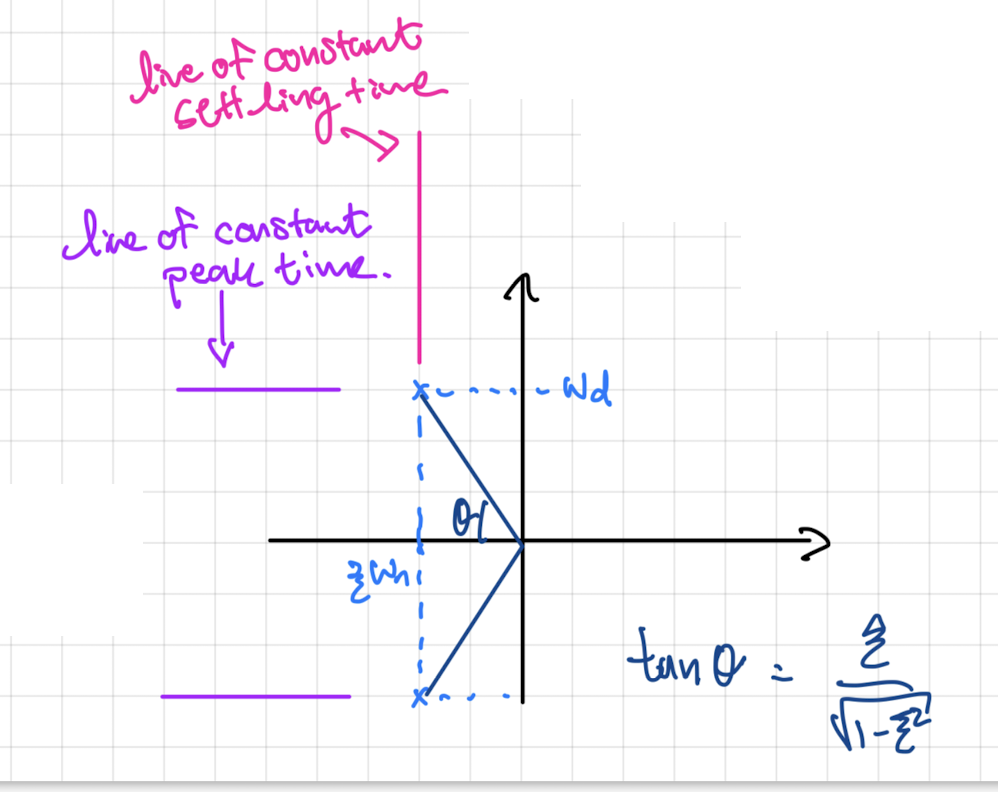
\includegraphics[width=0.4\textwidth]{images/pole_times_drawing.png}
\end{center}

\mheader{Poles}
\gap
\sheader{Assorted Rules about Poles}
\begin{enumerate}
\item A pole in the input function generates the forced response.
\item A pole in the transfer function generates the natural response.
\item The further to the left a pole is on the negative real axis, the faster the
  transient response will decay to zero.
\item The zeroes and poles generate the amplitude for both the forced and natural responses.
\item The position of the poles determines the systems peak time and settling time.
\item Repeated poles on the imaginary axis guarantee stability.
\end{enumerate}


\mheader{Reduction of Systems}
\begin{enumerate}
\item Cascade:
  \begin{center}
    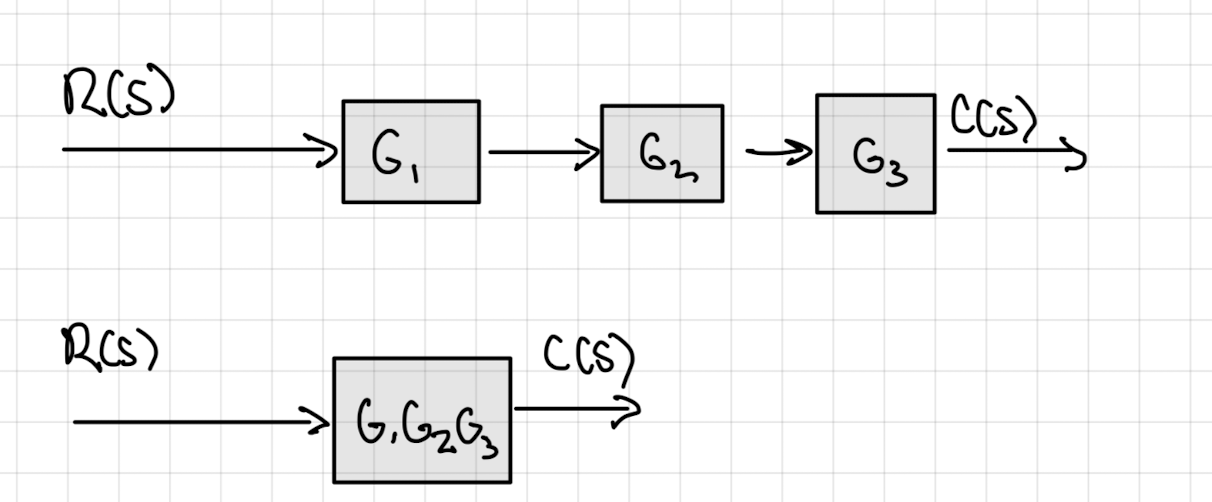
\includegraphics[width=0.5\textwidth]{images/cascade_blocks.png}
  \end{center}
\item Parallel:
  \begin{center}
    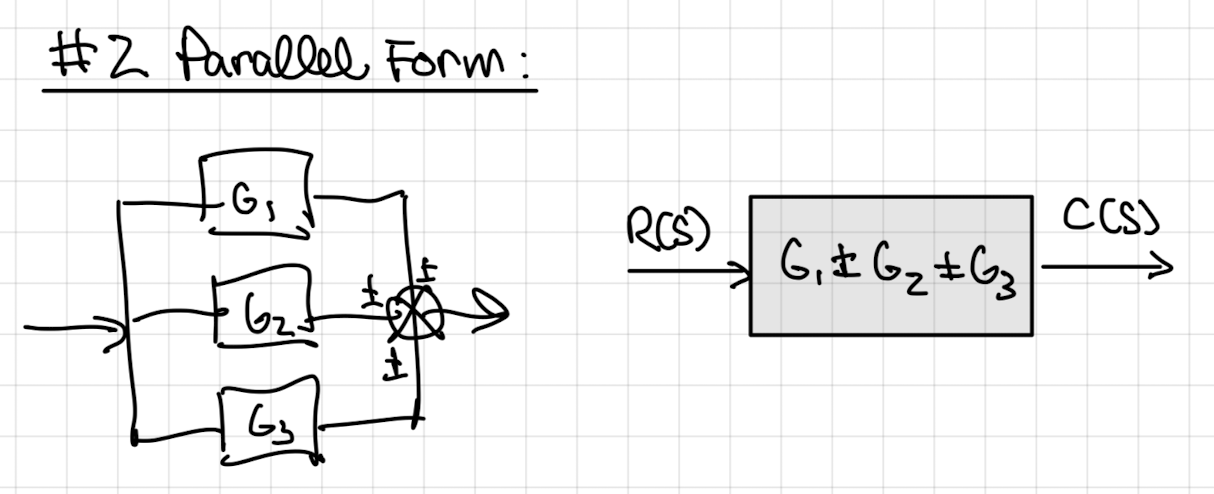
\includegraphics[width=0.5\textwidth]{images/parallel_blocks.png}
  \end{center}
\item Feedback:
  \begin{center}
    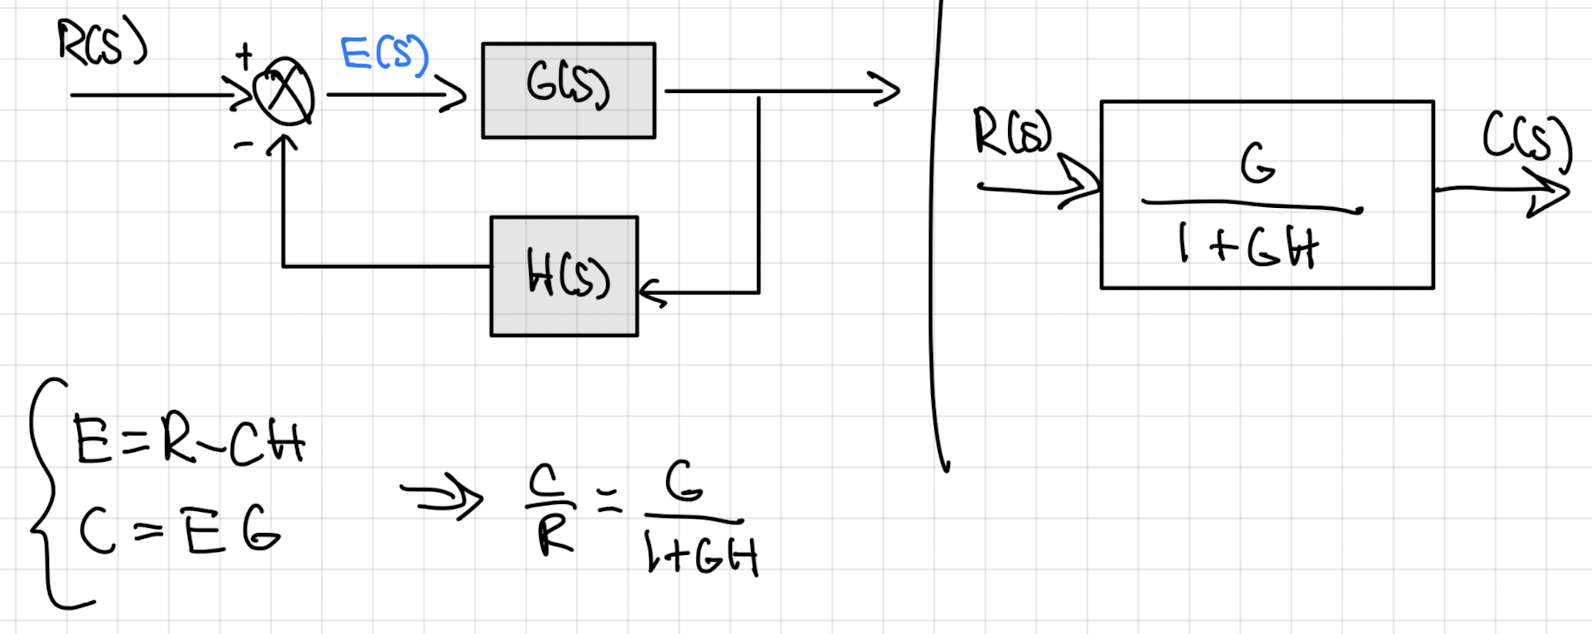
\includegraphics[width=0.5\textwidth]{images/feedback_blocks.png}
  \end{center}
\item Moving Blocks:
  \begin{center}
    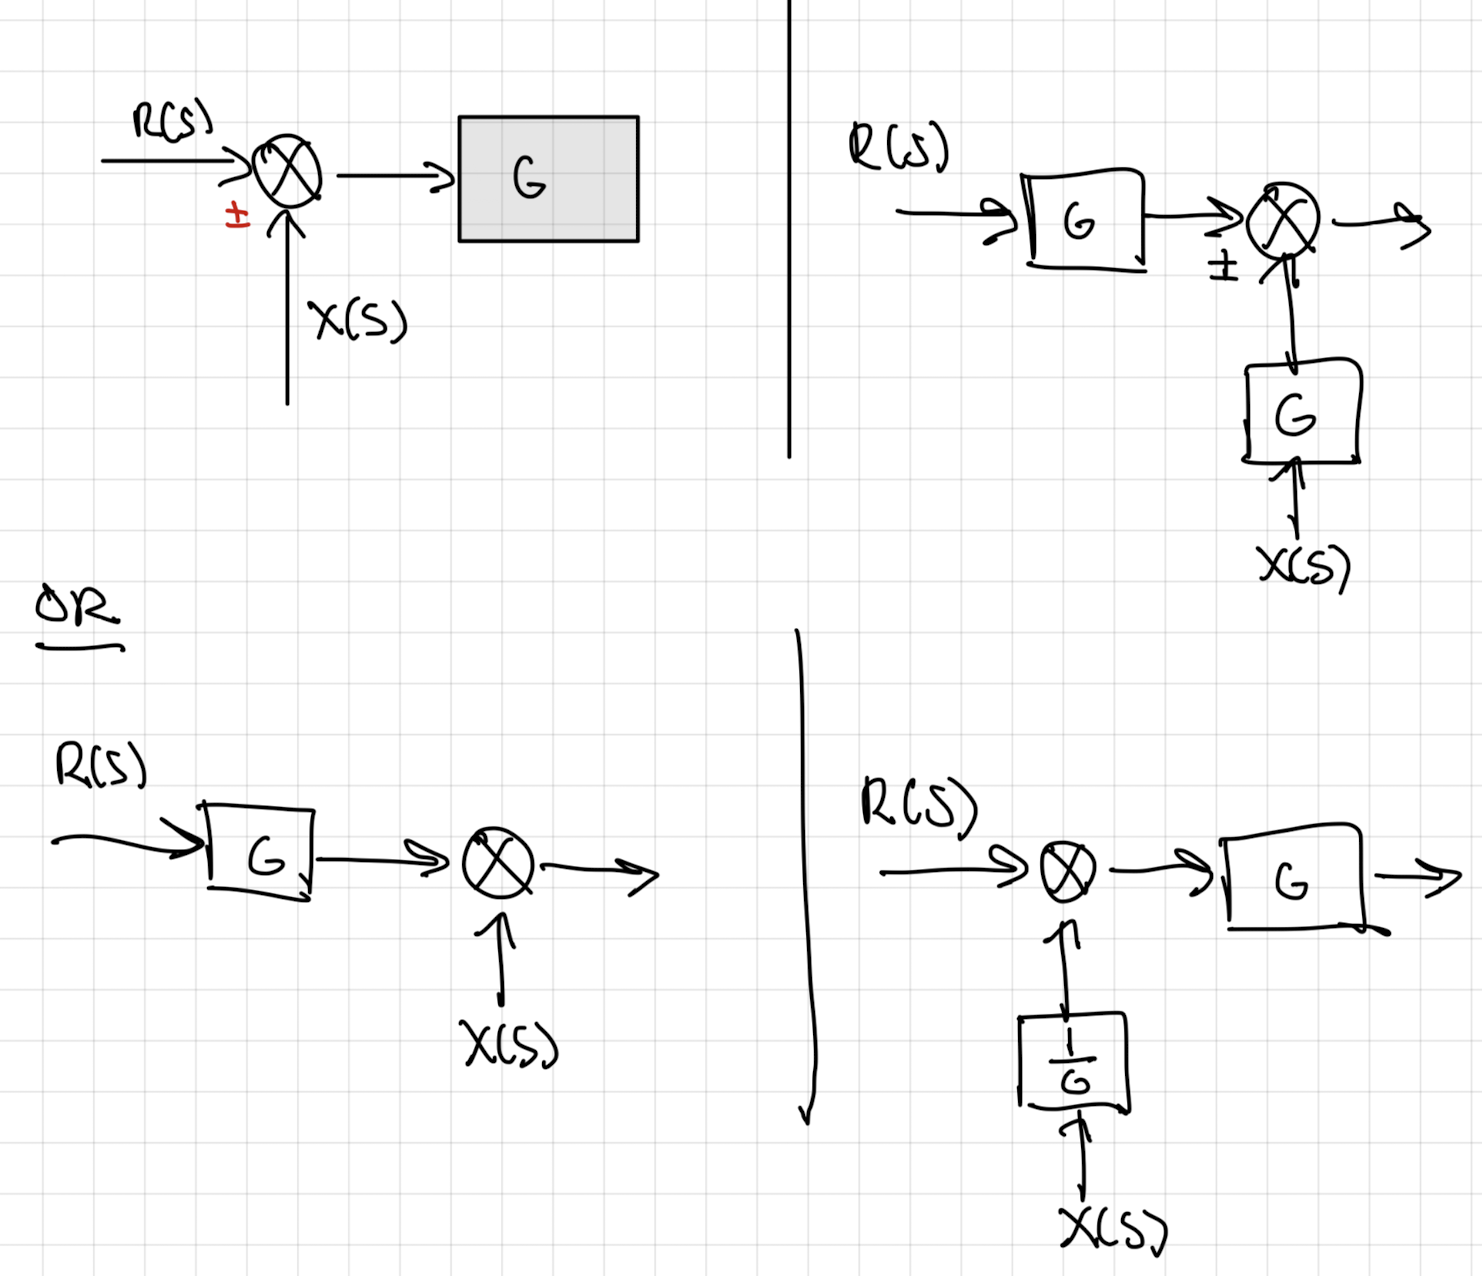
\includegraphics[width=0.5\textwidth]{images/moving_blocks.png}
  \end{center}
\end{enumerate}

\mheader{Routh-Hurwitz Criterion}
For a system with the following transfer function:
\begin{align*}
  H(s) = \frac{N(s)}{a_4s^4 + a_3s^3 + a_2s^2 + a_1s + a_0}
\end{align*}
\begin{center}
  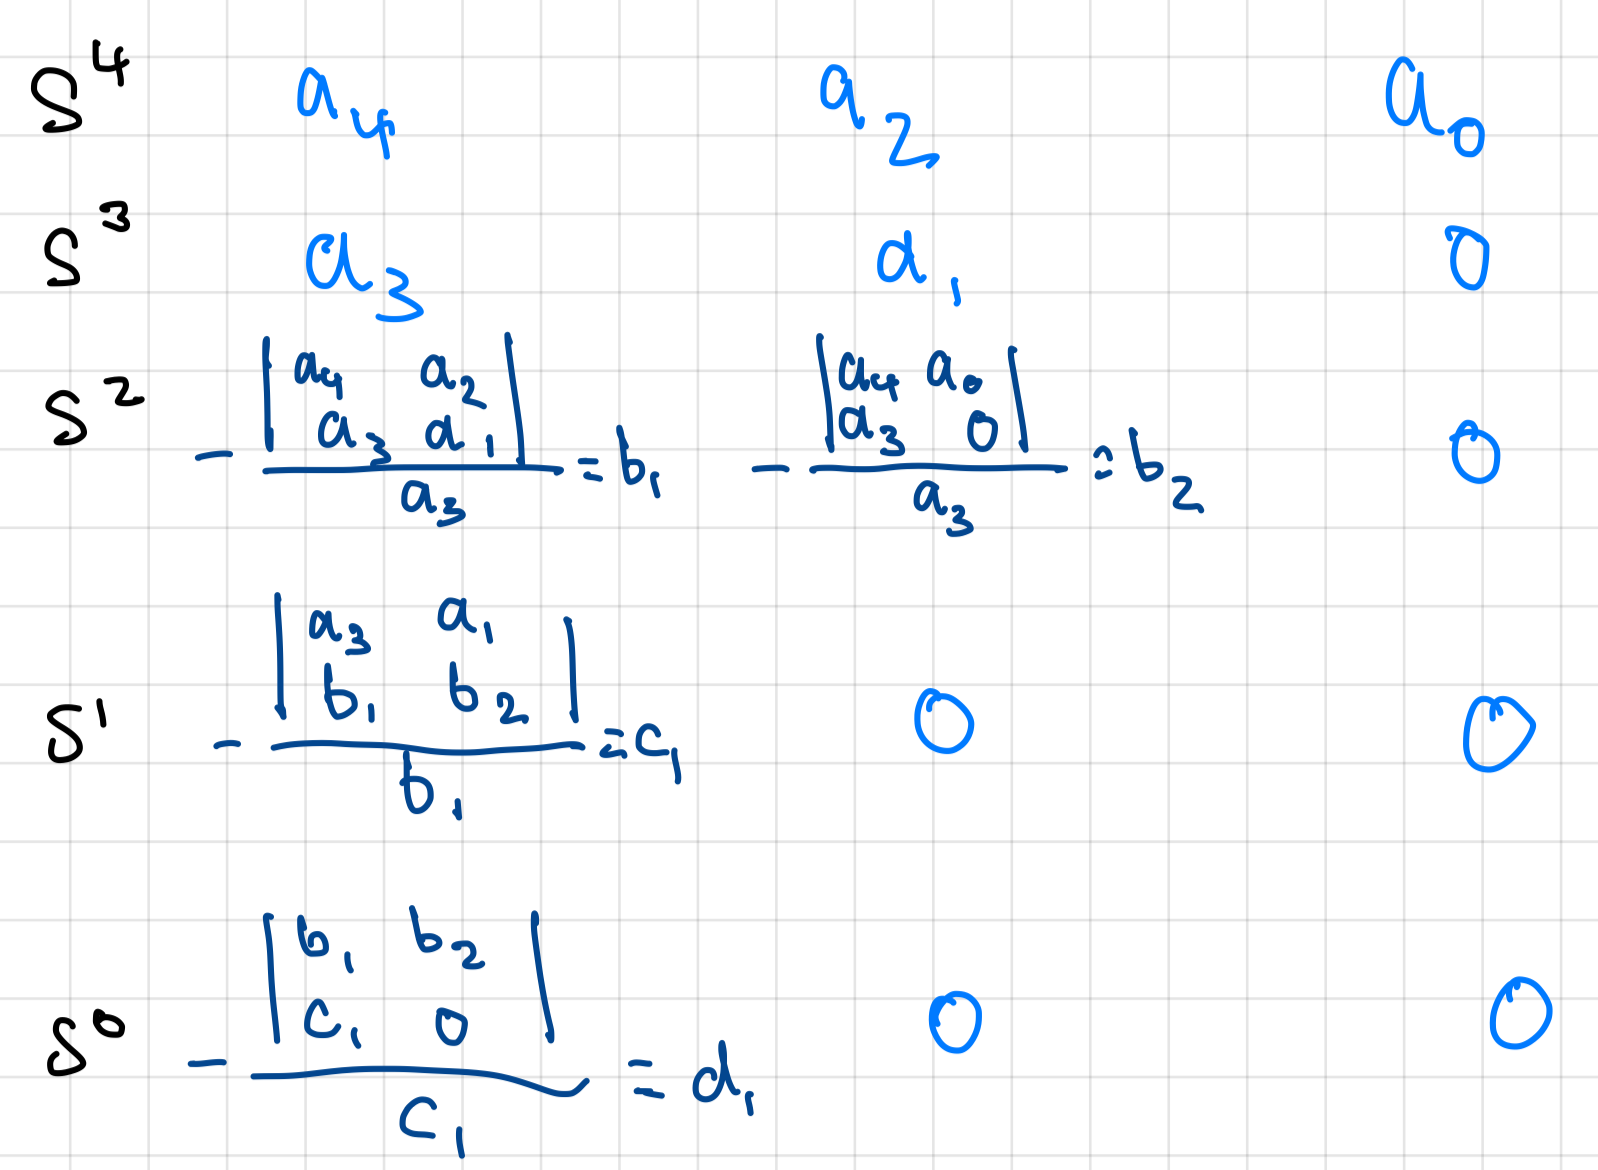
\includegraphics[width=0.5\textwidth]{images/routh_hurwitz.png}
\end{center}


\sheader{Routh-Hurwitz Edge Cases}
\begin{enumerate}
\item Zero in first column with non-zero numbers to the right.
  \begin{enumerate}
  \item Substitute the 0 for some $\epsilon$.
  \item At the end, take the limit $\epsilon \to 0$.
  \item If there are sign changes, the system is unstable and the number of ORHP poles are equal to the number of sign changes.
  \item If there are no sign changes, the system is marginally stable and there are at least two poles on the imaginary axis.
  \end{enumerate}
\item Zero for all entries in a row.
  \begin{enumerate}
  \item Using the powers from the column labels, take the derivative of the last non-zero row. This is called the \textit{auxillary polynomial}.
  \item Just yoss the resultant coefficients into the next row.
  \item As you were.
  \item If there is a zero row and no sign changes, then all the poles in the auxillary polynomial are on the imaginary axis and are symmetric. They also correspond to the roots of the auxillary polynomial.
  \item Hence, the system is marginally stable.
  \end{enumerate}
\end{enumerate}

\header{Useful Methods of System Analysis}
\mheader{Lagrangian Mechanics}
\begin{align*}
  \frac{d}{dt} \left(\frac{dT}{d\dot{q}}\right) + \frac{dU}{dq} + \frac{dR}{d\dot{q}} = \text{external forces}
\end{align*}

\mheader{Motors}

Motors have the following transfer function:
\begin{align*}
  \frac{\Theta(s)}{E(s)} = \frac{\kappa}{s(s+a)}.
\end{align*}

Which can be found using the following equations:
\begin{align*}
  \frac{T_\text{stall}}{e_a} &= \frac{k_t}{R} & k_b &= \frac{e_a}{\omega_\text{no-load}} & k = \frac{k_t}{RJ} &&  a &= \frac{1}{J}\left(\frac{k_t}{R}k_b + D\right)
\end{align*}

\begin{center}
---  midterm cutoff ---
\end{center}

\vfill \pagebreak

\header{Steady-State Analysis}

\sheader{Final Value Theorem} For some function $f(t)$ with Lagrange transform $\mathcal{L}\curly{f(t)} = F(s)$, then it follows that:
\begin{align*}
  \lim_{t \to \infty} f(t) = \lim_{s \to 0}s F(s).
\end{align*}

Generally, steady-state analysis is done on closed-loop systems with unity feedback (Figure \ref{fig:steady-state} with $H(s) = 1$). Hence, we can derive the error in the following manner:
\begin{align*}
  E(s) = \frac{R(s)}{1 + G(s) H(s)}
\end{align*}
And hence, to find the steady state error, take the limit as $\lim_{s\to 0 } sE(s)$.

\begin{figure}[htbp]
  \centering
  \begin{center}
    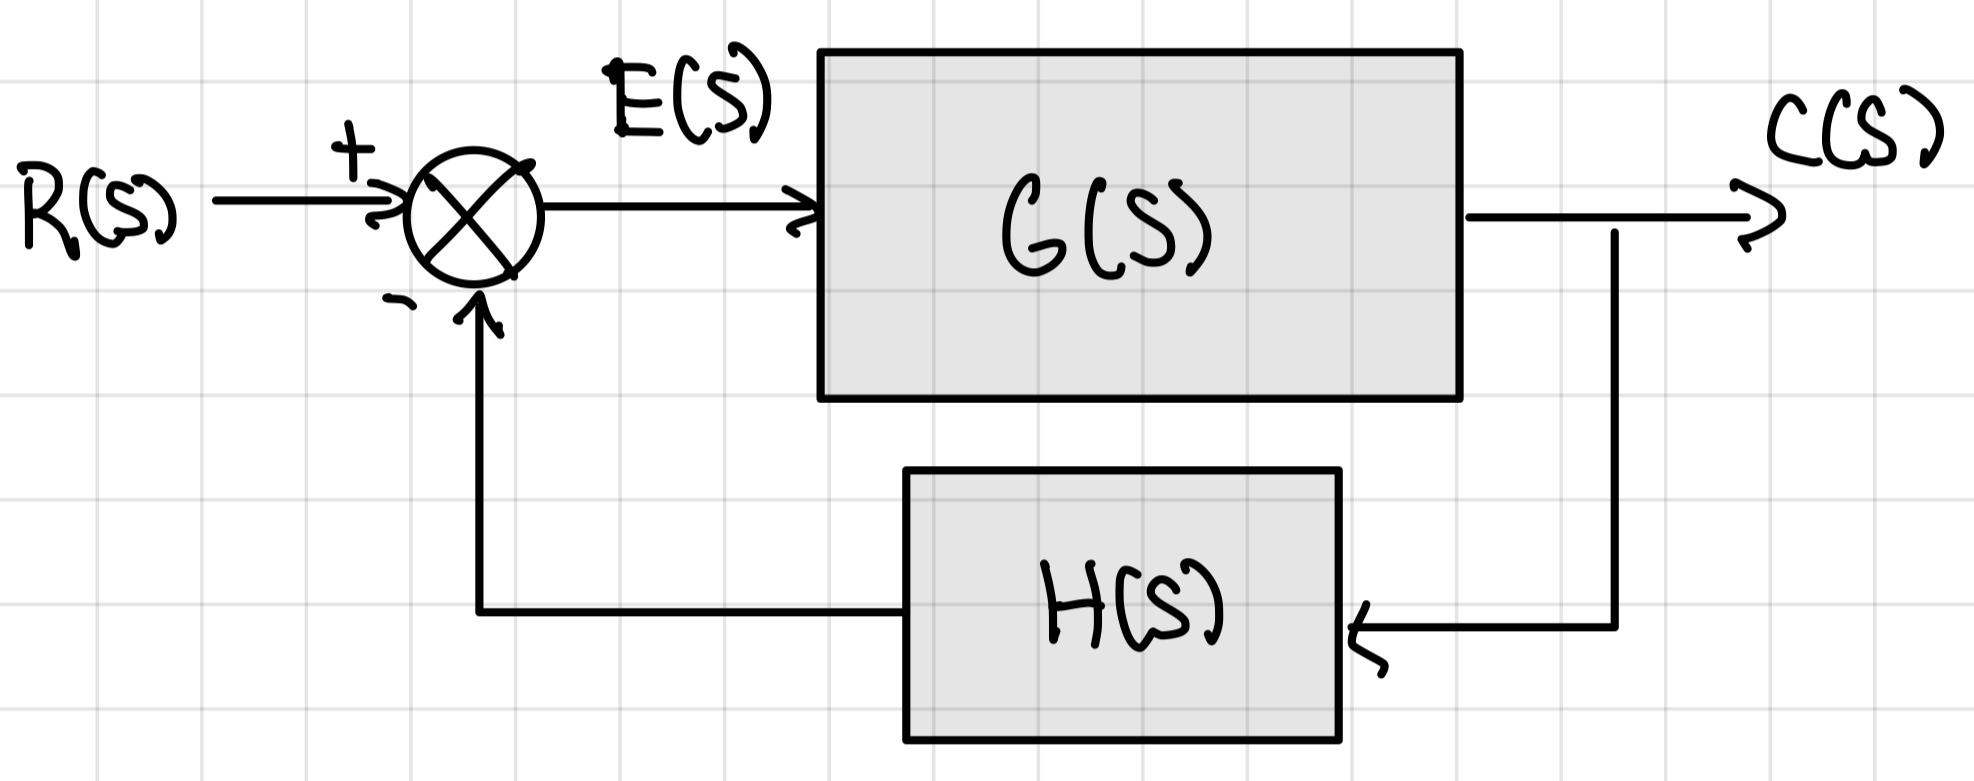
\includegraphics[width=0.5\textwidth]{images/standard_diagram.png}
  \end{center}
  \caption{Generic System}
  \label{fig:steady-state}
\end{figure}

Given this, for different inputs, there are conditions on the number of ``pure integrators'' in a system (i.e. the degree of the denominator). The condition is that:
\gap
\textit{For an input to a system $\ds R(s) = \frac{1}{s^n}$, then the denominator of the system must have degree $\geq n$.}
\gap
\sheader{Static Error Constants} For a system with unity feedback ($H(s) = 1$), then we can
define the ``static error constants'' for it. They are as follows:
\begin{itemize}
\item Position Constant: $\ds K_p = \lim_{s \to 0} G(s)$
\item Velocity Cosntant: $\ds K_v = \lim_{s \to 0} sG(s)$
\item Acceleration Cosntant: $\ds K_a = \lim_{s \to 0} s^2G(s)$  
\end{itemize}
As these constants increase, the value of the steady-state error decreases. One can apply these generally to systems with $H(s) \neq 1$ by doing the analysis with $G(s) \to G(s)H(s)$.
\gap
\header{Root Locus}
The Root Locus is a graphical presentation of how the locations of the closed-loop poles for a given system change as a system parameter is varied. It is a powerful method of analysis and design for stability and tranisent response.
\gap
Take for example some system with a gain coefficient $K$. As one changes $K$, one can analyze how the poles of the system change. By plotting those poles as $K$ changes, one can analyze the behaviour of the system under changing $K$. By plotting the root locus, one can answer several questions about how changing $K$ impacts the system, such as:
\begin{itemize}
\item How does the overshoot OS change?
\item How does $\omega_n$ and $\omega_d$ change?
\end{itemize}

\sheader{Hacking} It wouldn't be a mech course if there wasn't some strange way of trying to shortcut doing the full procedure. We can determine whether a point is on the root locus of a system, and what $K$ it corresponds to in the following way for some system $T(s)$:
\begin{align*}
  T(s) = \frac{KG}{1 + KGH}
\end{align*}

\begin{enumerate}
\item The poles occur for $1 + KGH = 0$, and thus, $KGH = -1$. This corresponds to a phase of $(2k + 1)\cdot 180^\circ$, $k \in \mathbb{Z}$. Thus, it follows that:
  \begin{align*}
    |KGH| &= 1 & \angle KGH = (2k + 1)\cdot 180^\circ & K = \frac{1}{|GH|}
  \end{align*}
\item In order to verify that it is on the root locus, check whether:
  \begin{align*}
    \angle KGH \in \curly{(2k + 1) \cdot 180^\circ : k \in \mathbb{Z}}
  \end{align*}
\item Then, if so, find the $K$ for which the point corresponds to:
  \begin{align*}
    K = \frac{1}{|GH|}
  \end{align*}
\end{enumerate}

\begin{figure}[htbp]
  \centering
  \begin{center}
    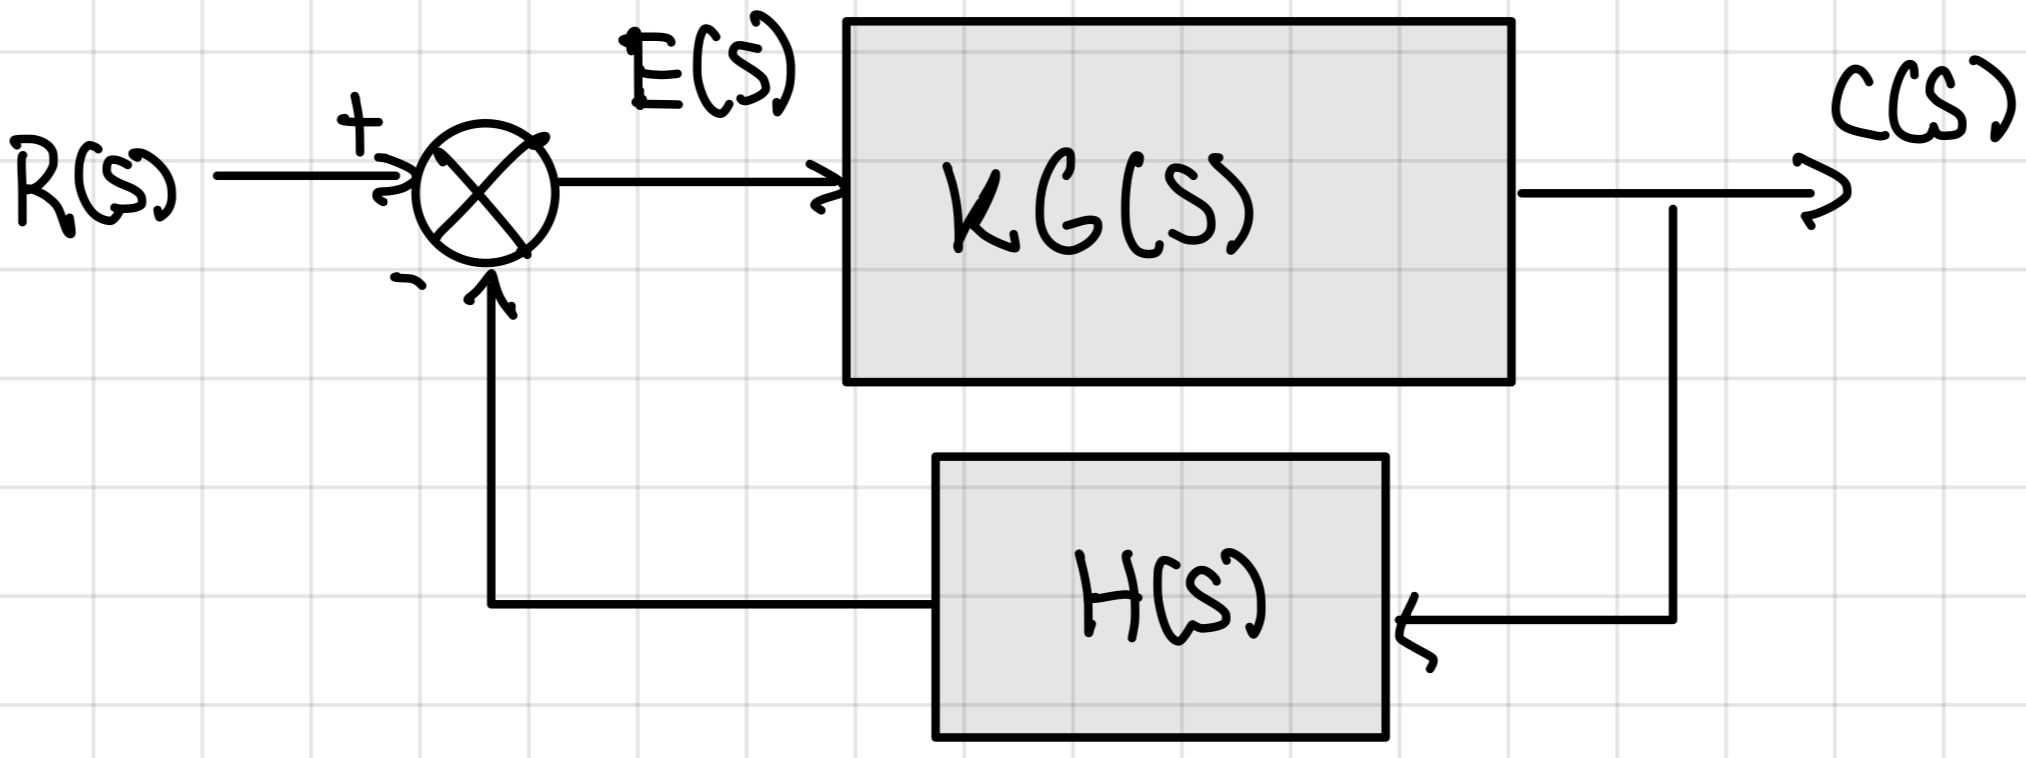
\includegraphics[width=0.5\textwidth]{images/with_gain.png}
  \end{center}
  \caption{Generic System with Gain $K$}
  \label{fig:with-gain}
\end{figure}

\header{Bode Plots/Frequency Response}

We call the transfer function of a system with $s = j\omega$ the \textit{frequency response function} (FRF). It can help to determine how a system responds to different frequency inputs. The FRF has two main components that are analyzed:
\begin{itemize}
\item \sheader{Gain} $\ds M = |G(j\omega)| = \sqrt{\text{Re}^2 + \text{Im}^2}$
\item \sheader{Phase} $\ds \phi = \angle G(j\omega) = \arctan \left(\frac{\text{Im}}{\text{Re}}\right)$
\end{itemize}
These can both be plotted in a \underline{Bode Plot}:
\begin{enumerate}
\item \sheader{Plot 1 (Gain)}
  \begin{itemize}
  \item $x$ axis: input frequency $w$, log scale
  \item $y$ axis: gain in decibels: $\ds M' = 20 \log(M)$
  \end{itemize}
\item \sheader{Plot 2 (Phase)}
  \begin{itemize}
  \item $x$ axis: input frequency $w$, log scale
  \item $y$ axis: phase $\phi$, normal scale, degrees.
  \end{itemize}
\end{enumerate}

\sheader{Properties of Bode Plots}
\begin{itemize}
\item Multiplication \to\, Summation: if $G(s) = N(s)P(s)$ then:
  \begin{itemize}
  \item Gain Plot is the sum of the $N(s)$ and $P(s)$ gain plots.
  \item Phase plot is the sum of the $N(s)$ and $P(s)$ gain plots.
  \end{itemize}
\item Inverse: if $G(s) = 1/N(s)$ where $N(s)$ is some known function:
  \begin{itemize}
  \item Gain Plot is the negative $N(s)$ gain plot.
  \item Phase Plot is the negative $N(s)$ gain plot.
  \end{itemize}
\end{itemize}

\header{Nyquist Plots}
The Nyquist plot examines how the open-loop transfer functions transforms a contour spanning the right-half plane in the $s$ domain into the ``$F$'' domain. The open-loop transfer function is given by $G(s)H(s)$ for some generic system like in Figure \ref{fig:steady-state}. This is useful computing the \textit{Nyquist Criterion}.
\gap
\sheader{Nyquist Criterion} Let:
\begin{itemize}
\item $Z$ be the number of closed-loop poles in the right-half plane.
\item $P$ be the number of open-loop poles in the right-half plane.
\item $N$ be the number of counter-clockwise revolutions around the point $(-1, 0)$ in the Nyquist plot.
\end{itemize}
Then, if $Z = 0$, then the system is stable.
\gap
\sheader{Plotting the Nyquist Plot}
\begin{enumerate}
\item Find the following four points:
  \begin{enumerate}
  \item $\omega = 0$
  \item $\omega = \infty$
  \item Imaginary Intercepts ($\text{Re} = 0$)
  \item Real Intercepts ($\text{Im} = 0$)
  \end{enumerate}
\item Draw the points, and them connect them in the following order, assuming no duplicate
  points:
  \begin{enumerate}
  \item $\omega = 0$
  \item Imaginary Intercepts ($\text{Re} = 0$)
  \item Real Intercepts ($\text{Im} = 0$)
  \item $\omega = \infty$
  \end{enumerate}
\item Mirror it across the real axis.
\end{enumerate}
Then, using the open-loop transfer function, one can calcualte $P$, and then deduce $N$ from the Nyquist Plot. If the loop passes through $-1$, then it is generally decided that the system is ``marginally stable''.
\gap
\header{Controllers}
A control system consists of certain subsystems assembled for the purpose of obtaining a desired output, with desired performance, given a specific input. One can move the position of zeroes and poles of a system to change its performance. One can also \textit{compensate} a system by adding extra zeroes and poles. This is called controller/compensator design.
\gap
In a PID system, we can do the following:
\begin{itemize}
\item Multiply the error by $k_p$ before feeding it back into the system.
\item Take the cumulative total error over a period and multiply it by a constant $k_i$.
\item Take the rate of change in error and multiply it by a constant $k_d$.
\end{itemize}
Mathematically, this looks like:
\begin{align*}
  &\mathcal{L} \curly{k_p e(t) + k_i \int e(t) dt + k_d \frac{de(t)}{dt}}\\
  &\left[k_p + \frac{k_i}{s} + k_d s\right]E(s)
\end{align*}
Generally, it is known that:
\begin{itemize}
\item Differentiation improves transient response (overshoot, settling time).
\item Integration improves steady-state error.
\end{itemize}
Hence, one can induce this with different types of controllers:
\begin{itemize}
\item \sheader{PI Controller} Proportional control and integral control
  \begin{align*}
    k_p + \frac{k_i}{s} = \frac{k_p \left(s + \frac{k_i}{k_p}\right)}{s}
  \end{align*}
  \begin{itemize}
  \item Generates a pole at the origin and a zero at $\ds -\frac{k_i}{k_p}$.
  \item It improves the steady state error.
  \end{itemize}
\item \sheader{PD Controller} Proportional and derivative control
  \begin{align*}
    k_p + k_ds = k_d \left(s + \frac{k_p}{k_d}\right)
  \end{align*}
  \begin{itemize}
  \item Generates a zero at $\ds -\frac{k_p}{k_d}$
  \item It improves the transient response (OS, settling time)
  \end{itemize}
\end{itemize}
Another class of controllers are \textit{Lead/Lag Controllers}. They have the general form of:
\begin{align*}
  \frac{s + z_c}{s + p_c}
\end{align*}
\begin{itemize}
\item \sheader{Lag Controllers}
  \begin{itemize}
  \item Zero and pole close to the origin: $z_c, p_c \approx 0$.
  \item Zero smaller than pole: $|z_c| < |p_c|$.
  \item Improves steady-state error.
  \end{itemize}
\item \sheader{Lead Controllers}
  \begin{itemize}
  \item Zero and pole far from the origin $|z_c|, |p_c| \gg 0$.
  \item Zero larger than pole: $|z_c| > |p_c|$.
  \item Improves transient response.
  \end{itemize}
\end{itemize}
\sheader{Design Process}
\begin{itemize}
\item An engineer always designs first for Transient Response, and then Steady-State error after.
\item The process is meant to be iterative, i.e. T, SS, T, SS,...
\item If one first designs a PD controller, then a PI controller, it is called a PID controller.
\item If one first designs a Lead and then a Lag compensator, the resulting controller is called a Lead-Lag compensator.
\end{itemize}

We can also rewrite everything to be in terms of Lag/Lead compensators:

\begin{center}
\renewcommand{\arraystretch}{2} % Adjust this value to increase/decrease spacing
\begin{tabular}{|c|c|}
\hline
\textbf{Controller} & \textbf{Function} \\
\hline
PI & $\ds K \frac{s + z_c}{s}$ \\
\hline
Lag & $\ds K \frac{s + z_c}{s + p_c}$ \\
\hline
PD & $\ds K (s + z_c)$ \\
\hline
Lead & $\ds K \frac{s + z_c}{s + p_c}$ \\
\hline
PID & $\ds K \frac{(s + z_\text{lag})(s + z_\text{lead})}{s}$ \\
\hline
Lag-Lead & $\ds K \frac{(s + z_\text{lag})(s + z_\text{lead})}{(s + p_\text{lag}) (s + p_\text{lead})}$\\
\hline
\end{tabular}
\end{center}

We can also do this all in the form of op-amps:

\begin{figure}[H]
  \centering
  \begin{center}
    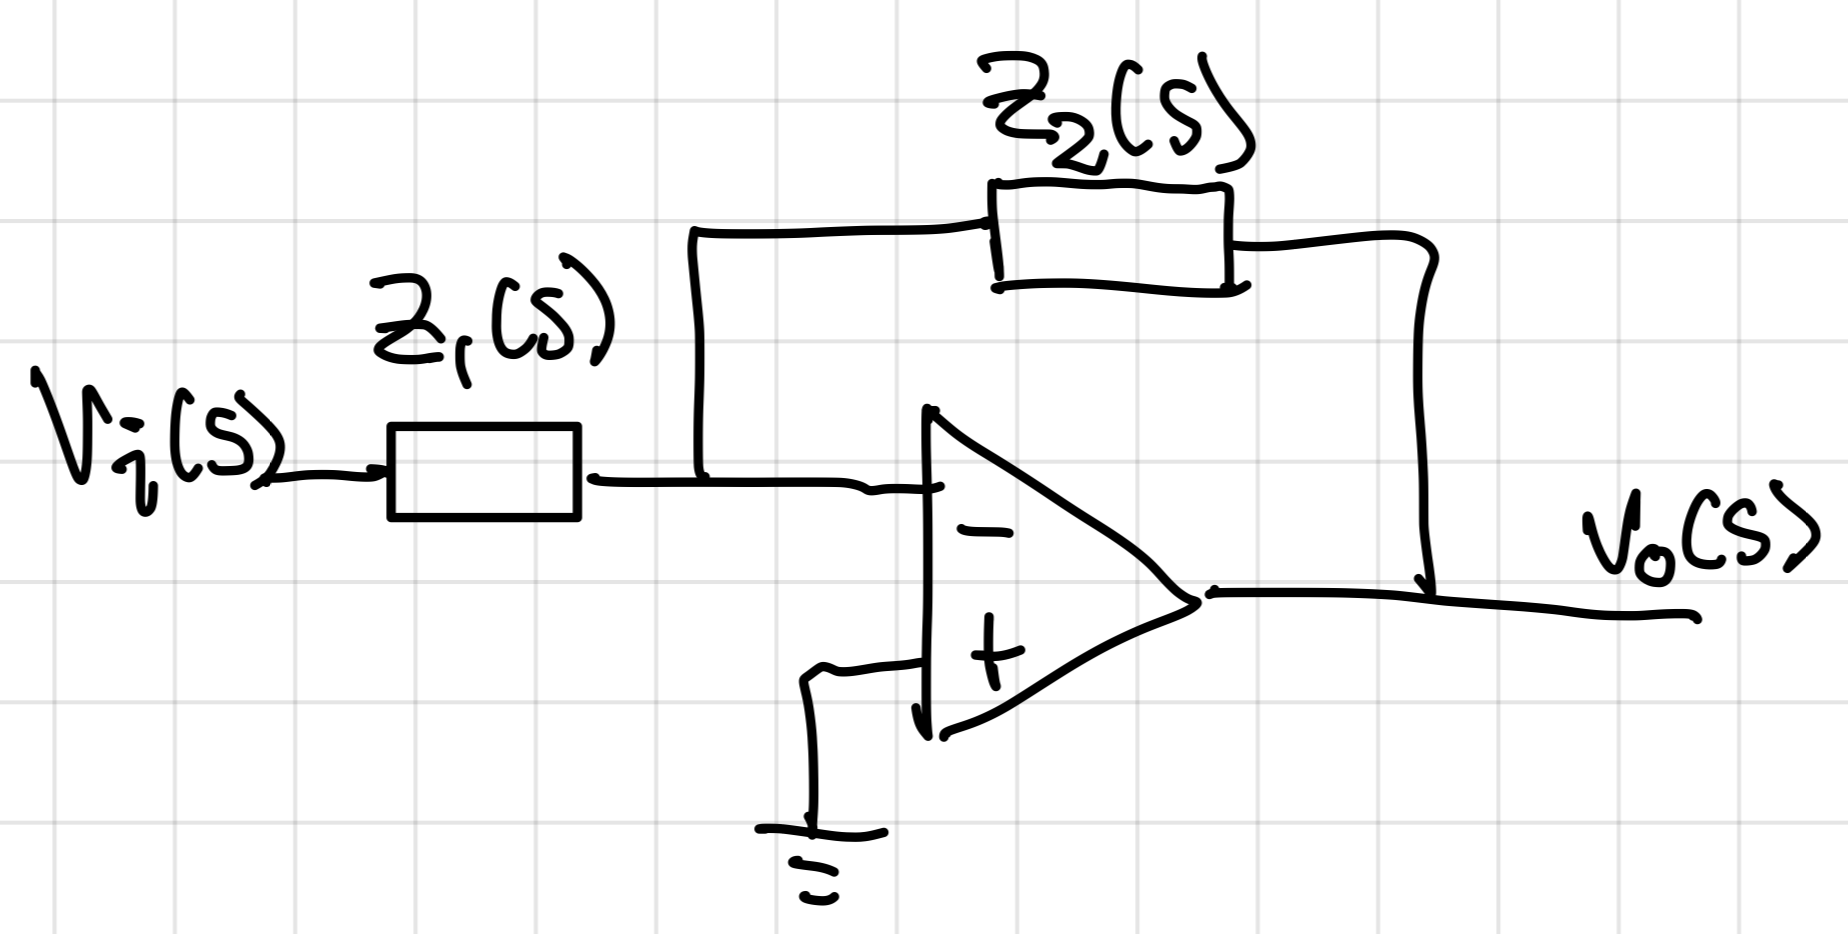
\includegraphics[width=0.5\textwidth]{images/generic_opamp.png}
  \end{center}
  \caption{Generic Opamp}
  \label{fig:opamp}
\end{figure}

And so to create controllers out of impedances $Z$, we can do the following:

\begin{center}
\begin{tabular}{|c|c|c|c|}
\hline
Controller Type & Z1 Element & Z2 Element & Function \\
\hline
PI & \begin{circuitikz}
  \draw (0,0)
    to[R=$R_1$] (3,0);
\end{circuitikz} & 
\begin{circuitikz}
  \draw (0,0) 
    to[R=$R_2$] (2,0)
    to[C=$C$] (4,0);
\end{circuitikz} & $\ds -\frac{R_2}{R_1} \frac{ \left(s + \frac{1}{R_2C}\right)}{s}$ \\
\hline
PD & \begin{circuitikz}
  % Left wire in
  \draw (0,0) to[short, o-*] (1,0);

  % Vertical to top for capacitor
  \draw (1,0) to[short] (1,2)
               to[C=$C$] (3,2)  % Capacitor on top branch
               to[short] (3,0);

  % Bottom branch: resistor
  \draw (1,0) to[R=$R_1$] (3,0); % Resistor on bottom branch

  % Right wire out
  \draw (3,0) to[short, -*, o-] (4,0);
\end{circuitikz} & \begin{circuitikz}
  \draw (0,0) 
    to[R=$R_2$] (3,0);
\end{circuitikz} &  $\ds -R_2 C \left(s + \frac{1}{R_1 C}\right)$\\
\hline
PID & \begin{circuitikz}
  % Left wire in
  \draw (0,0) to[short, o-*] (1,0);

  % Vertical to top for capacitor
  \draw (1,0) to[short] (1,2)
               to[C=$C_1$] (3,2)  % Capacitor on top branch
               to[short] (3,0);

  % Bottom branch: resistor
  \draw (1,0) to[R=$R_1$] (3,0); % Resistor on bottom branch

  % Right wire out
  \draw (3,0) to[short, -*, o-] (4,0);
\end{circuitikz} & \begin{circuitikz}
  \draw (0,0) 
    to[R=$R_2$] (2,0)
    to[C=$C$] (4,0);
\end{circuitikz} &  $\ds - \left[ \left(\frac{R_2}{R_1} + \frac{C_1}{C_2}\right) + R_2C_1s + \frac{1}{R_1C_2 s}\right] $\\
\hline
\end{tabular}
\end{center}

and also this (I'm lazy)

\begin{figure}[H]
  \centering
  \begin{center}
    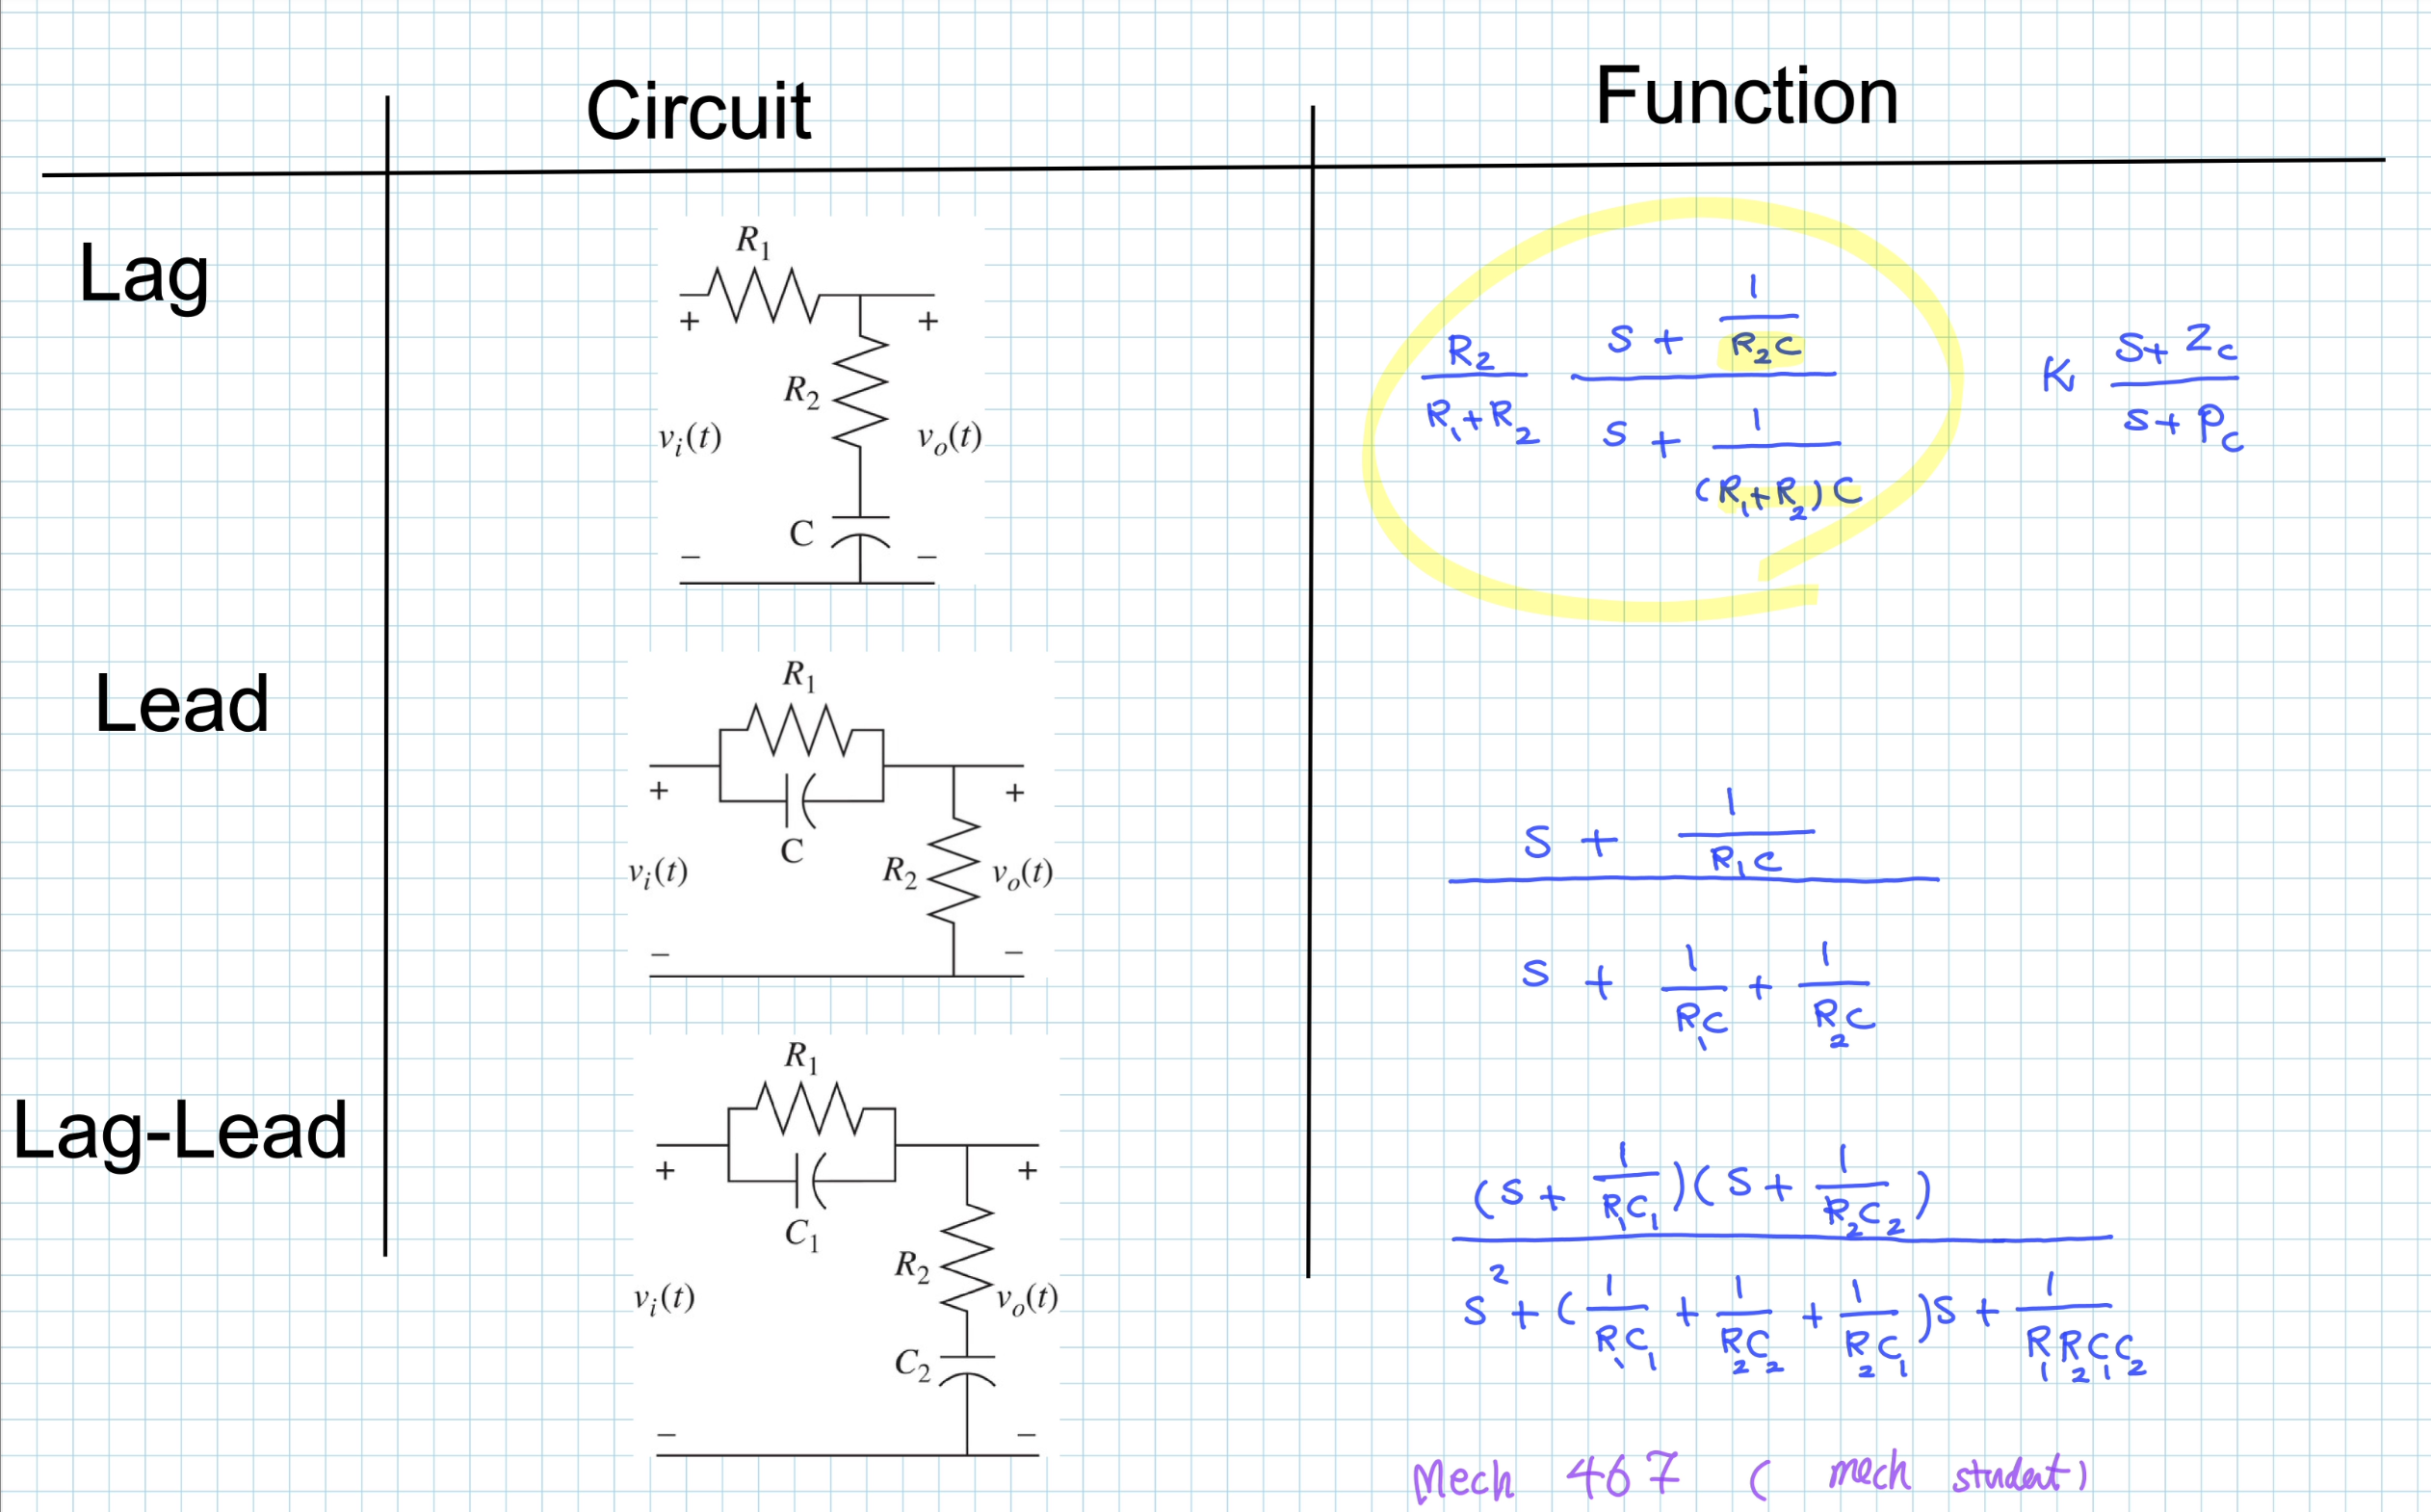
\includegraphics[width=\textwidth]{images/lazy.png}
  \end{center}

  \caption{Lazy}
  \label{fig:lazy}
\end{figure}



\end{document}
